\subsection{出力部}
出力部は風景生成部で生成したパノラマ画像とデータ取得部で取得したユーザ情報を元に風景,他ユーザの表示,またユーザの移動による風景の更新を行う処理群である. ユーザ A とユーザ Bがレクリエーションしている出力例を図\ref{figure:output}に示す.
(a),(b)はそれぞれ ユーザ A, ユーザ Bが実際にいる場所の風景である.(c) はユーザ A, ユーザ Bが遠隔旅行こーすとして設定した場所(東京)の風景を示している.(d)は ユーザ A, ユーザ Bが実際にいる場所と, 指定した遠隔地の位置関係である. (e)はユーザ Aから見える風景である.現実空間に遠隔地が重畳され,同じ遠隔地を指定したユーザ Bのアバターが表示されている.(f)は反対にユーザ Bから見える風景である. (g)はシステム使用時の遠隔地における二人のユーザの位置関係である.

\begin{figure*}[ht]
\begin{center}
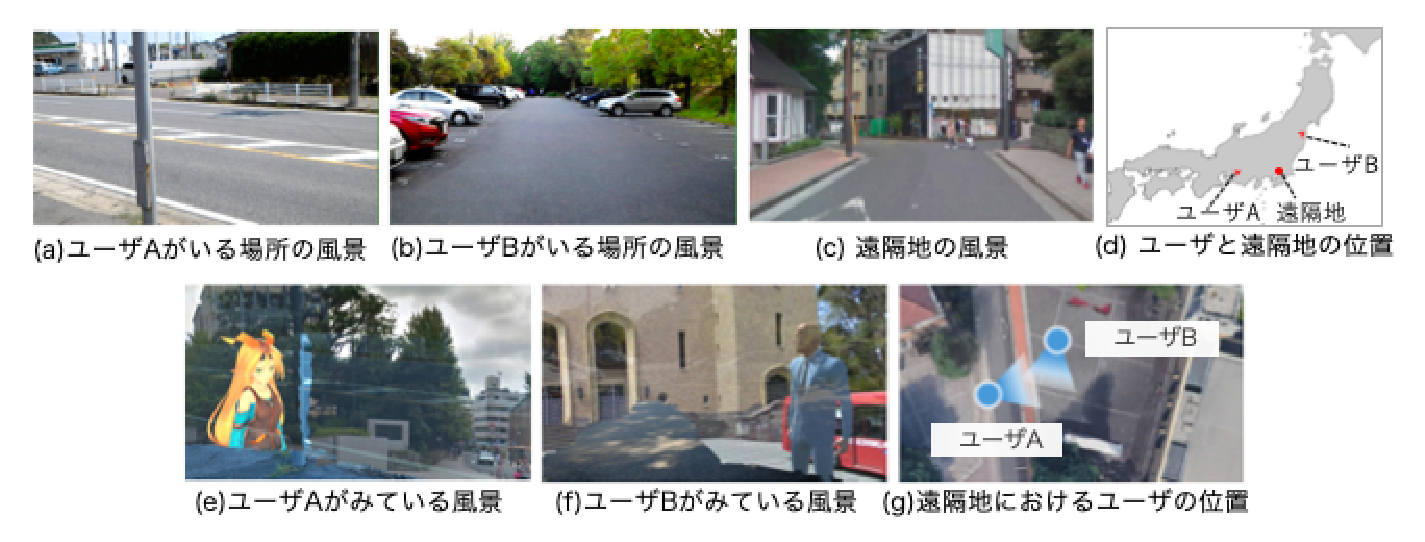
\includegraphics[width=17cm]{img/04_detail/output.eps}
\end{center}
\caption{システム使用例と出力}
\label{figure:output}
\end{figure*} 

\subsubsection{風景表示}
現実風景への重畳は球体のオブジェクトにテクスチャとして風景生成部で生成したパノラマ画像を貼り付けることで行う.
パノラマ画像を貼り付けた球体オブジェクトの内部にシステム起動時ユーザの視点となるUnityのカメラオブジェクトを配置する.
これにより周囲の風景は遠隔地の風景へと変化する.


\clearpage

\subsubsection{他ユーザの表示}
他ユーザの表示ではユーザが表示している遠隔地が近い他ユーザのアバターを表示する.アバターとしてUnityのAsset Storeで無料配布されているUnityちゃんを使用した\cite{unitychan}.
ユーザ間のアバターの同期処理にはオンラインゲームの同期処理に使われる Photon Unity Cloud を利用した\cite{photon}.
表示するユーザはデータ取得部で生成したJSONデータを元に決定する.
システムはJSONデータのユーザ情報と現在地情報から,表示する遠隔地同士の距離が近いユーザのユーザIDを取得する.
そして取得したユーザIDを元にPhoton Unity Cloud のルームを検索する.ユーザは取得した近いユーザのIDと同じ名前のルームが存在する場合,入室する.検索した結果近いユーザのIDと同じ名前のルームがなければシステムは自身のユーザIDと同名のルームを作成する.
これにより他ユーザとのアバターの共有を行う.
アバターの向きはHololensの
$\it{y}$
軸方向のみ同期していおり,図 \ref{figure:abatar}(a)のようにアバターの回転を水平方向のみに制限している.またアバターの座標はHololensの座標と同期しており,図\ref{figure:abatar}(b)のようにユーザが進行した方向に動く.

\begin{figure}[h]
\begin{center}
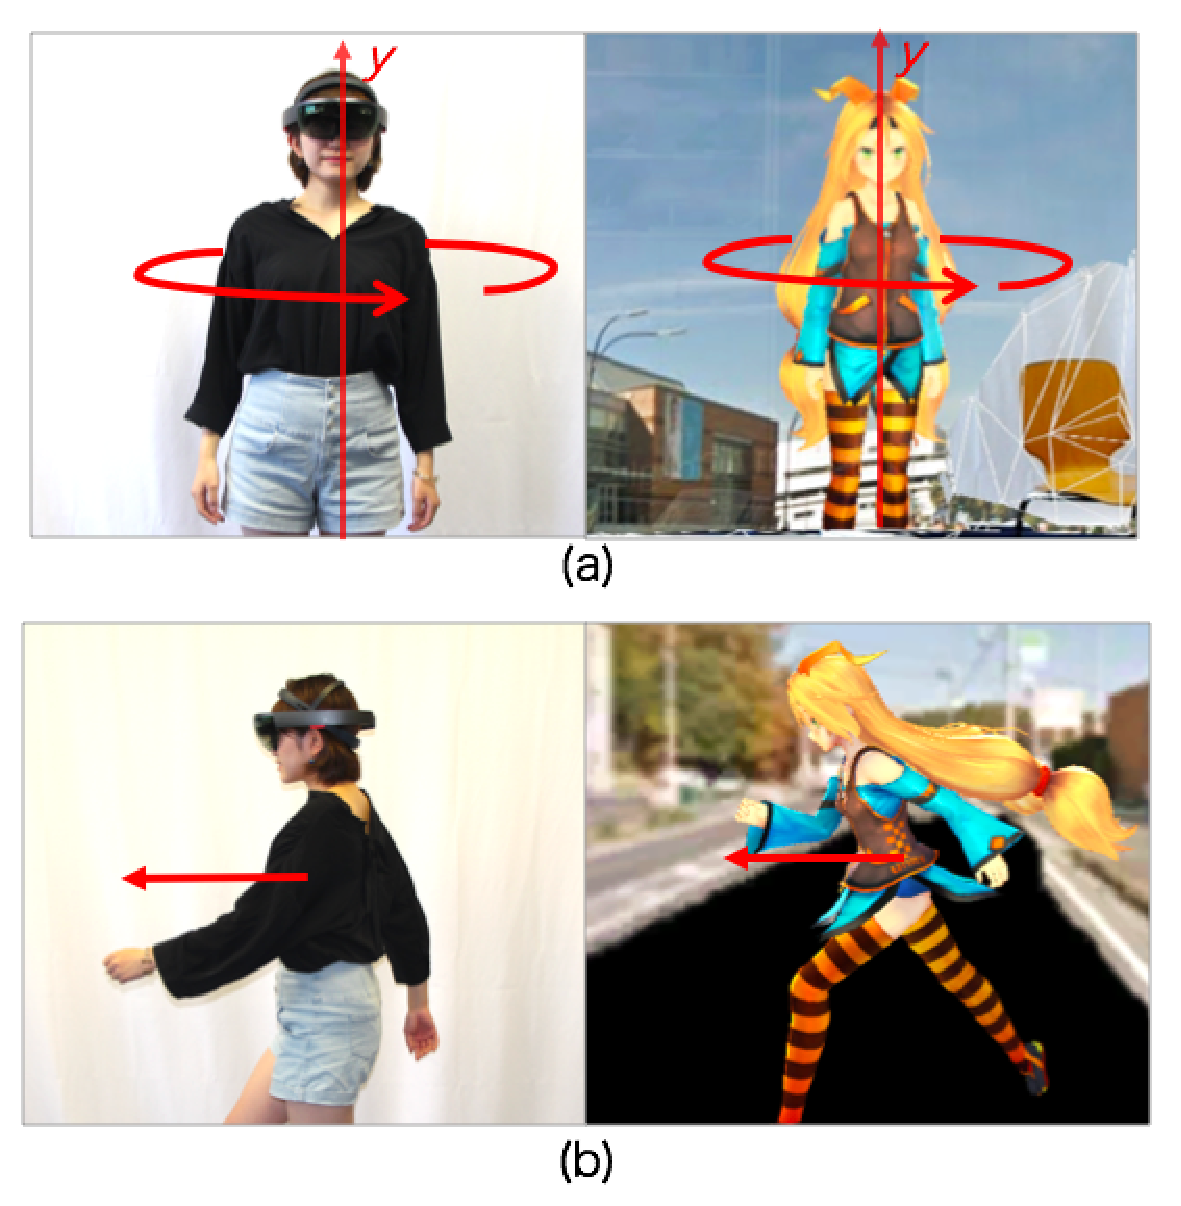
\includegraphics[width=11cm]{img/04_detail/avatar_move.eps} 
\end{center}
\caption{アバターの動き}
\label{figure:abatar}
\end{figure} 

\clearpage

\subsubsection{風景更新}
風景更新ではユーザが歩くことでパノラマ画像を更新する.ユーザの位置はHololens の自己位置推定機能によって算出する.自己位置推定機能とはHololensのアプリケーション起動時の座標との相対距離を推定する機能である. HololensとUnityのカメラオブジェクトは座標と方向が同期されているため,カメラオブジェクトの座標を取得することで自己位置を推定が可能である.風景の更新はHololensが3メートル座標移動するごとに行う.これはGoogle が定めた StreetView 認定要件において StreetView 間の距離が3 メートルとなっていたためである.
システムは風景更新時のHololensの座標と,前回の更新時のHololensの座標から移動方向を算出し,ユーザの移動方向に道が続くように風景表示用の球体オブジェクトを回転させる.
移動方向の算出にはUnityのVector3クラスに定義されている,GetAim関数により算出できる.